
\documentclass[10pt]{beamer} % die 10pt sollten festgelegt bleiben, da dies die Groesse 
%der Mathematikschrift etc. beeinflusst


\usepackage[utf8]{inputenc} % nicht im template
\usepackage[ngerman]{babel}  
\usepackage{hyperref} 
%\usepackage{colortbl} % wird schon im template geladen


\usepackage[ief,footuniheadings, headframesubtitle]{./unirostock/beamerthemeRostock}
% erster Parameter: Farbschema
%        moegliche Werte (nomen est omen): uni, inf, msf, ief, mnf, mef, juf, wsf, auf, thf, phf
%        Standardwert: uni
% zweiter Parameter: Fusszeile
%        moegliche Werte: footuni (Standard) - Fusszeile nach Handbuch des CD
%                         foottitle          - Autor und Title in der Fusszeile
%                         footheadings       - lebende Ueberschriften in der Fusszeile
%                         footuniheadings    - Autor und Uni sowie lebende Ueberschriften in der Fusszeile
% dritter Parameter: Kopfzeile
%        moegliche Werte: headlogo (Standard)- Inhalt von \mylogo in der Kopfzeile
%                         headtitle          - Vortragstitel
%                         headframetitle     - Folientitel
%                         headframesubtitle  - Folientitel und -untertitel
%        bitte nicht mehrere Varianten gleichzeitig angeben :-)

%%%%%%%%%%%% Festlegung der Titelseite %%%%%%%%%%%%%%%%%%%%%%%%%%%%%%%%%
\title{Service- and Security Monitoring}

\subtitle{Auswertung, Konsolidierung, Korrelierung und Visualisierung
IT-Sicherheitskritischer Ereignisse\\}

\author{\textsc{Martin Steinbach}}

\date{30.05.2018}

\institute{Universität Rostock, Institut für Informatik\\\\}

\titlegraphic{\textbf{Seminar Sommersemester 2018}\\ Auswertung und
Visualisierung komplexer Daten}

% ein alternatives Titelbild kann mittels 
%\titleimage{Dateiname.xyz}
% angegeben werden (auf vernuenftiges Seitenformat und Kontrastwerte achten, Skalierung und Abschneiden der oberen rechten Ecke passieren automatisch)


%%%%%%%%%%%% Festlegungen fuer Kopf- und Fusszeile %%%%%%%%%%%%%%%%%%%%
% Institutsname f\"ur die Fusszeile (nur wenn bei Paketeinbindung 'footuni' angegeben ist)
%\footinstitute{Institut für Informatik}
% eigenes Logo oben rechts hinzufuegen (bitte auf vernuenftiges Format achten - ein zu hohes Logo verschiebt das Layout)
\renewcommand{\mylogo}{
\includegraphics[width=18.5mm]{institutslogo}}


%%%%%%%%%%%%%%%%%% Los geht's %%%%%%%%%%%%%%%%%%%%%%%%%%%%%%%%%%%%%%%%%
%%%%%%%%%%%%%%%%%%%%%%%%%%%%%%%%%%%%%%%%%%%%%%%%%%%%%%%%%%%%%%%%%%%%%%%
\begin{document}


%%%%%%%%%%%%%%%%%%%%%%%%%%%%%%%%%%%%%%%%%%%%%%%%%%%%%%%%%%%%%%%%%%%%%%%
%%%%%%%%%%%%%%%%%%%%%%%%%%%%%%%%%%%%%%%%%%%%%%%%%%%%%%%%%%%%%%%%%%%%%%%
\begin{frame}% Titelseite
  \titlepage
\end{frame}


%%%%%%%%%%%%%%%%%%%%%%%%%%%%%%%%%%%%%%%%%%%%%%%%%%%%%%%%%%%%%%%%%%%%%%%
%%%%%%%%%%%%%%%%%%%%%%%%%%%%%%%%%%%%%%%%%%%%%%%%%%%%%%%%%%%%%%%%%%%%%%%
\begin{frame}{Struktur}
  \tableofcontents[pausesections]
\end{frame}


%%%%%%%%%%%%%%%%%%%%%%%%%%%%%%%%%%%%%%%%%%%%%%%%%%%%%%%%%%%%%%%%%%%%%%%
%%%%%%%%%%%%%%%%%%%%%%%%%%%%%%%%%%%%%%%%%%%%%%%%%%%%%%%%%%%%%%%%%%%%%%%
\section{Einführung}
%%%%%%%%%%%%%%%%%%%%%%%%%%%%%%%%%%%%%%%%%%%%%%%%%%%%%%%%%%%%%%%%%%%%%%%
%%%%%%%%%%%%%%%%%%%%%%%%%%%%%%%%%%%%%%%%%%%%%%%%%%%%%%%%%%%%%%%%%%%%%%%

%%%%%%%%%%%%%%%%%%%%%%%%%%%%%%%%%%%%%%%%%%%%%%%%%%%%%%%%%%%%%%%%%%%%%%%
\subsection{Warum Überwachung?}
%%%%%%%%%%%%%%%%%%%%%%%%%%%%%%%%%%%%%%%%%%%%%%%%%%%%%%%%%%%%%%%%%%%%%%%
\begin{frame}
    \frametitle{Warum Überwachung?}
    \framesubtitle{Servicemonitoring = Securitymonitoring?}
    
    \pause
    
   \begin{exampleblock}{Ziele der Informationssicherheit}
        \begin{itemize}
            \item   Vertraulichkeit
            \item   \textbf{Verbindlichkeit}
            \item   \textbf{Integrität}       
            \item   \textbf{Verfügbarkeit}
        \end{itemize}     
   \end{exampleblock}
    \pause
    \begin{exampleblock}{Betrachtungen}
        \begin{itemize}
            \item Zeitliche Perspektive
            \item Schweregrad (severity)
            \item Quelle
            \item Ereigniskorrelation
        \end{itemize} 
    \end{exampleblock}
            
\end{frame}

\begin{frame}
\frametitle{Warum Überwachung?}
\framesubtitle{Schaden identifizieren und vermeiden}

    \begin{itemize}
        \item 90\% aller Firmen: Opfer von Cyberattacken
        \item 80\% derer mit finanziellen Einbußen
        \item Diebstahl geistigen Eigentums (zwischen 2011 und 2015 Verdopplung) 
    \end{itemize}

\end{frame}

\begin{frame}
    \frametitle{Warum Überwachung?}
        \framesubtitle{Servicemonitoring = Securitymonitoring?}
        
        \begin{alertblock}{\centering Servicemonitoring = Securitymonitoring?}
            \vspace{0.3cm}
            \centering{ \Large{ Ja!?}}
            \vspace{0.3cm}
            
            Nur ein unmanipulierter Dienst, der erwiesenermaßen seine
            Aufgaben erfüllt, hält die Ziele der IT-Sicherheit ein.\\
            \vspace{0.3cm}
        \end{alertblock}     
    
        \pause
           
        \begin{alertblock}{Beweis durch Überwachung}
             \begin{itemize}
                 \item Unerwartetes Verhalten
                 \item Erreichbarkeit
                 \item Angriffserkennung
                 \item Nachvollziebarkeit
             \end{itemize}
        \end{alertblock}
    

\end{frame}

%%%%%%%%%%%%%%%%%%%%%%%%%%%%%%%%%%%%%%%%%%%%%%%%%%%%%%%%%%%%%%%%%%%%%%%
\subsection{Überwachungsformen}
%%%%%%%%%%%%%%%%%%%%%%%%%%%%%%%%%%%%%%%%%%%%%%%%%%%%%%%%%%%%%%%%%%%%%%%
\begin{frame}
    \frametitle{Aktive Überwachung}
        \framesubtitle{Beispiel Sequenzdiagramm}
        
        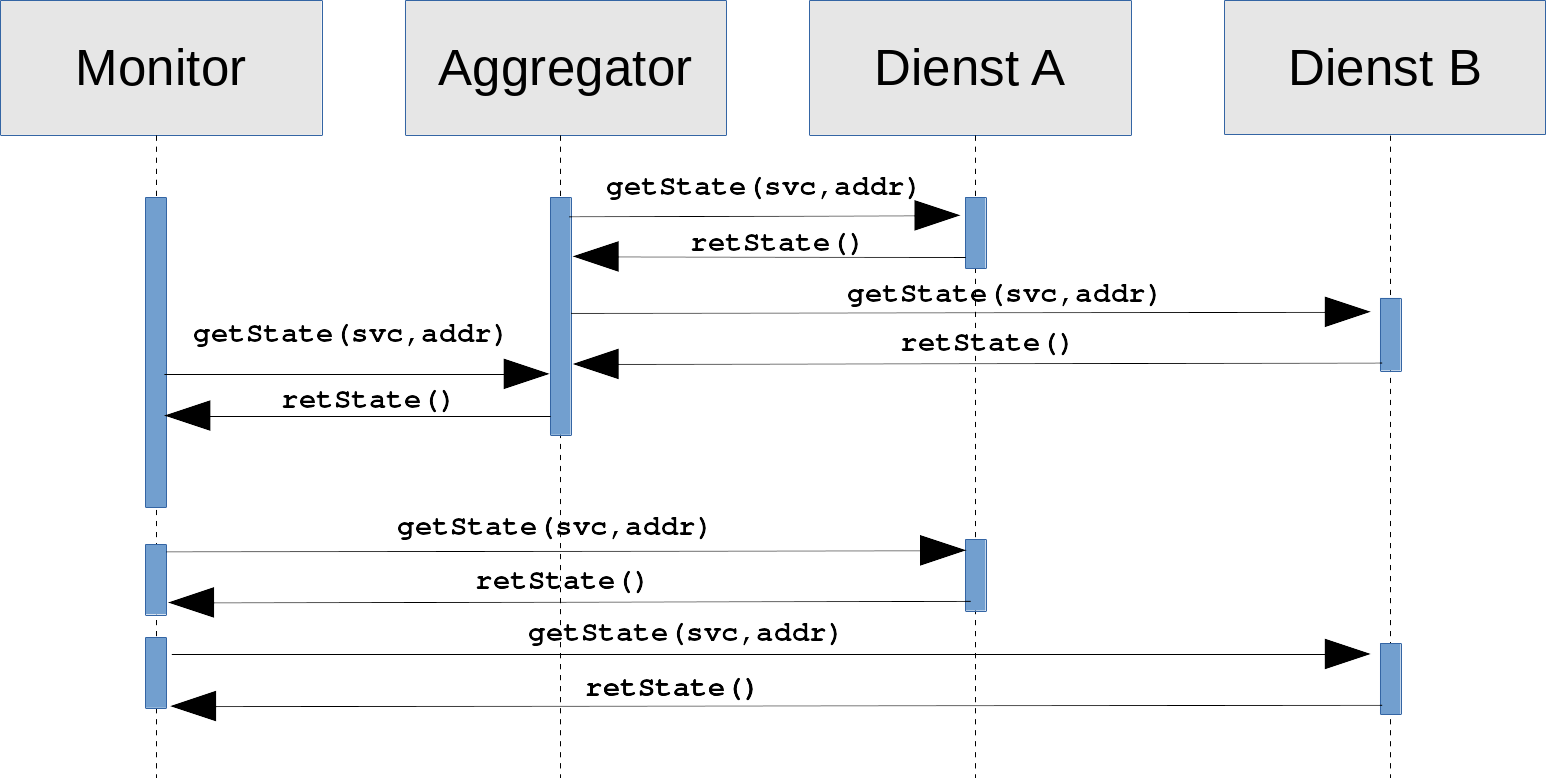
\includegraphics[scale=0.25]{img/sequence_uml_active_trans.png}

\end{frame}


\begin{frame}
\frametitle{Passive Überwachung}
\framesubtitle{Beispiel Sequenzdiagramm}

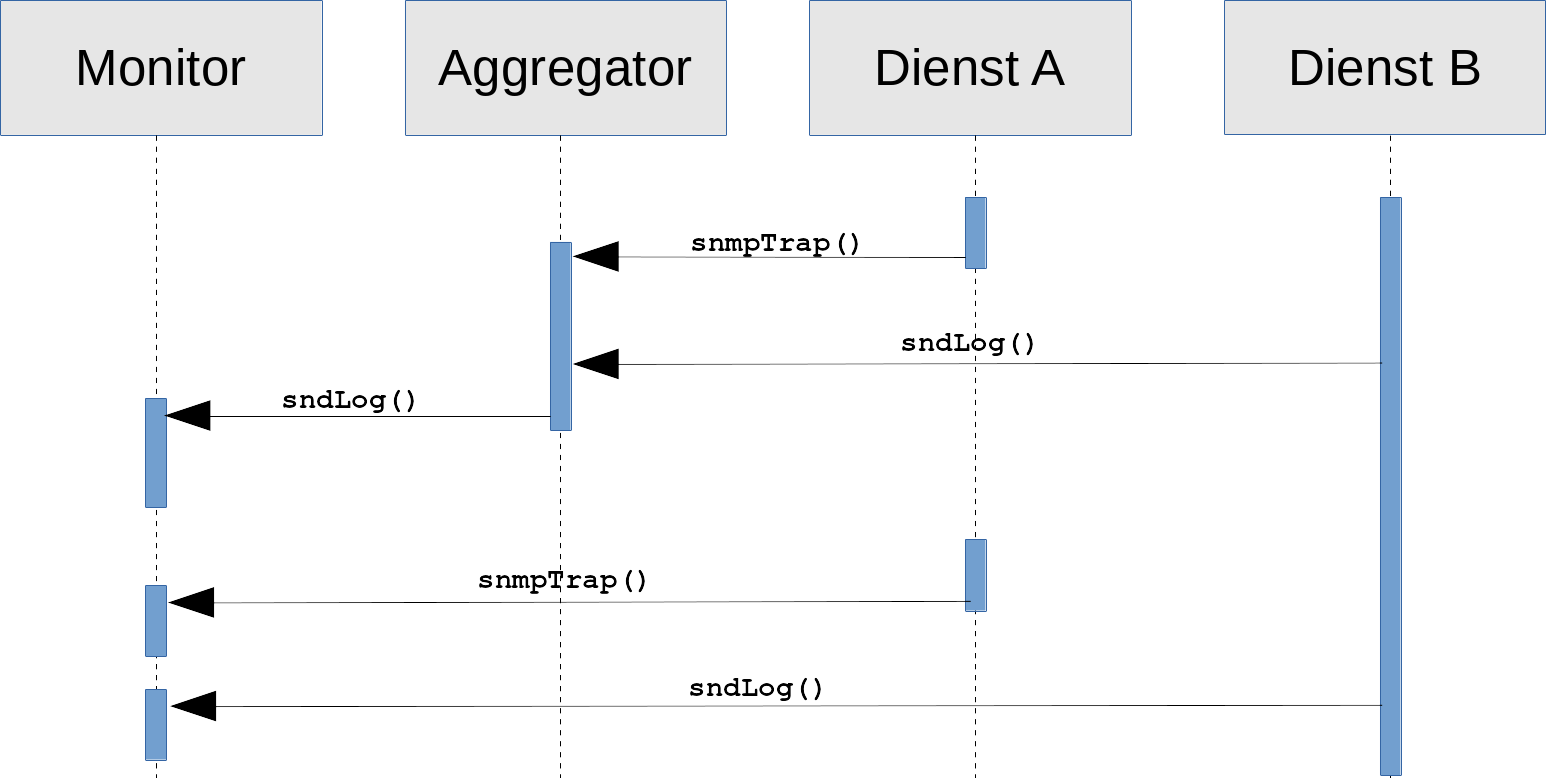
\includegraphics[scale=0.25]{img/sequence_uml_passive_trans.png}

\end{frame}

%%%%%%%%%%%%%%%%%%%%%%%%%%%%%%%%%%%%%%%%%%%%%%%%%%%%%%%%%%%%%%%%%%%%%%%
%%%%%%%%%%%%%%%%%%%%%%%%%%%%%%%%%%%%%%%%%%%%%%%%%%%%%%%%%%%%%%%%%%%%%%%
\section{Aktives Monitoring}
%%%%%%%%%%%%%%%%%%%%%%%%%%%%%%%%%%%%%%%%%%%%%%%%%%%%%%%%%%%%%%%%%%%%%%%
%%%%%%%%%%%%%%%%%%%%%%%%%%%%%%%%%%%%%%%%%%%%%%%%%%%%%%%%%%%%%%%%%%%%%%%

%%%%%%%%%%%%%%%%%%%%%%%%%%%%%%%%%%%%%%%%%%%%%%%%%%%%%%%%%%%%%%%%%%%%%%%
\subsection{Was kann überwacht werden}
%%%%%%%%%%%%%%%%%%%%%%%%%%%%%%%%%%%%%%%%%%%%%%%%%%%%%%%%%%%%%%%%%%%%%%%
\begin{frame}
\frametitle{Aktive Überwachung}
\framesubtitle{Was kann überwacht werden?}

    \begin{alertblock}{}
        \centering{Jede Entität, deren Status deutlich zueinander abgrenzbar sind.}
    \end{alertblock}

    \vspace{0.5cm}

    \begin{columns}
        \column{0.48\textwidth}
            \begin{itemize}
                \item Betriebsystem\color{red}abhängig
                    \begin{itemize}
                        \item Betriebsystemparameter
                        \begin{itemize}
                            \item   Auslastung
                            \item   Speicher
                            \item   Prozesse
                            \item   Datendurchsatz
                        \end{itemize}
                        \item Updates
                        \item Sicherheitsauditierung
                    \end{itemize}
             \end{itemize}
    
        \column{0.48\textwidth}
        \begin{itemize}
            \item Betriebsystem\color{red}unabhängig
            \begin{itemize}
                \item Netzwerkdienste
                \begin{itemize}
                    \item L3:   ICMP\{4,6\}
                    \item L4:   TCP, UDP - basierend
                    \item L4+:  SNMP
                \end{itemize}
                \item Sensoren
                \item Aktive Netzwerkkomponenten
            \end{itemize}
        \end{itemize} 
    \end{columns}




\end{frame}

\begin{frame}
\frametitle{Visualisierungen}
\framesubtitle{Statusverlauf}

    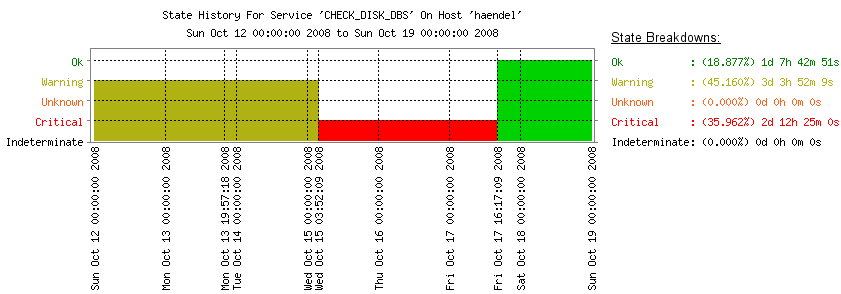
\includegraphics[scale=0.45]{img/nag_trend.png}
    \vspace{0.5cm}
    
    \footnoterule
    \footnotesize{
        Quelle:          selbst erstellt\\
        Erstellt mit:    NagVis}

\end{frame}
\begin{frame}
\frametitle{Visualisierungen}
\framesubtitle{packets/time}

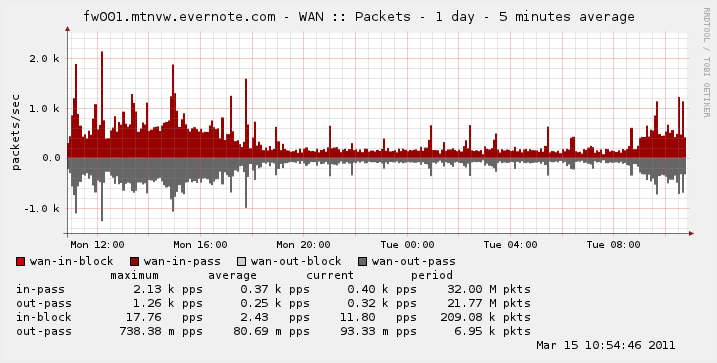
\includegraphics[scale=0.4]{img/status_rrd_graph_img.png}
\vspace{0.5cm}

\footnoterule
\footnotesize{
   Quelle:          https://redmine.pfsense.org/issues/1354\\
   Erstellt mit:    https://oss.oetiker.ch/rrdtool/}


\end{frame}
%%%%%%%%%%%%%%%%%%%%%%%%%%%%%%%%%%%%%%%%%%%%%%%%%%%%%%%%%%%%%%%%%%%%%%%
%%%%%%%%%%%%%%%%%%%%%%%%%%%%%%%%%%%%%%%%%%%%%%%%%%%%%%%%%%%%%%%%%%%%%%%
\section{Passives Monitoring}
%%%%%%%%%%%%%%%%%%%%%%%%%%%%%%%%%%%%%%%%%%%%%%%%%%%%%%%%%%%%%%%%%%%%%%%
%%%%%%%%%%%%%%%%%%%%%%%%%%%%%%%%%%%%%%%%%%%%%%%%%%%%%%%%%%%%%%%%%%%%%%%
\frame{\tableofcontents[currentsection]}

%%%%%%%%%%%%%%%%%%%%%%%%%%%%%%%%%%%%%%%%%%%%%%%%%%%%%%%%%%%%%%%%%%%%%%%
\subsection{Netzwerkanalyse}
%%%%%%%%%%%%%%%%%%%%%%%%%%%%%%%%%%%%%%%%%%%%%%%%%%%%%%%%%%%%%%%%%%%%%%%
\begin{frame}
\frametitle{Probing}
\framesubtitle{Korrelierung von Netzwerkscans}

\begin{alertblock}{\textit{scanning detection systems}}
    \begin{itemize}
        \item Trafficanalyse zu ungenau
        \item Erstellung eines \textit{fingerprints} kaum möglich
        \end{itemize}
\end{alertblock}

\begin{exampleblock}{\textit{Verkehrskorrelation durch statistische Verfahren}}
    \begin{itemize}
         \item Scans werden zeitlich korreliert
         \item Scan-Traffic zuordnung zu Scan-Technik
    \end{itemize}
\end{exampleblock}

\end{frame}

%%%%%%%%%%%%%%%%%%%%%%%%%%%%%%%%%%%%%%%%%%%%%%%%%%%%%%%%%%%%%%%%%%%%%%%
\subsection{Logkorrelation in Cloud-Umgebungen}
%%%%%%%%%%%%%%%%%%%%%%%%%%%%%%%%%%%%%%%%%%%%%%%%%%%%%%%%%%%%%%%%%%%%%%%
\begin{frame}
\frametitle{Cloud}
\framesubtitle{Anforderungen an eine Logkorrelation}

    \begin{block}{cloud}
        \begin{itemize}
            \item Stark steigende Systemanzahl (10K+)
            \item In wenigen Sekunden: virtuelles RZ
            \item Dynamisch wachsendes/sinkendes Logaufkommen
            \item Dynamische Kosten
            \item Proprietäre, inkompatible Monitoringsysteme
            \footnote{IETF-draft: \textit{Syslog Extension for Cloud Using Syslog 
            Structured Data}}
        \end{itemize}
    \end{block}
    \pause
    \begin{block}{Anforderungen Logkorrelation}
        \begin{itemize}
            \item Manuell undurchführbar
            \item Skalierbar (n+1)
            \item Automatisch durchführbar
            \item Minimierung des Speicheraufwandes
        \end{itemize}
    \end{block}

\end{frame}
%%%%%%%%%%%%%%%%%%%%%%%%%%%%%%%%%%%%%%%%%%%%%


\begin{frame}
\frametitle{Prototyp JCorrelat}
\framesubtitle{Schema}


 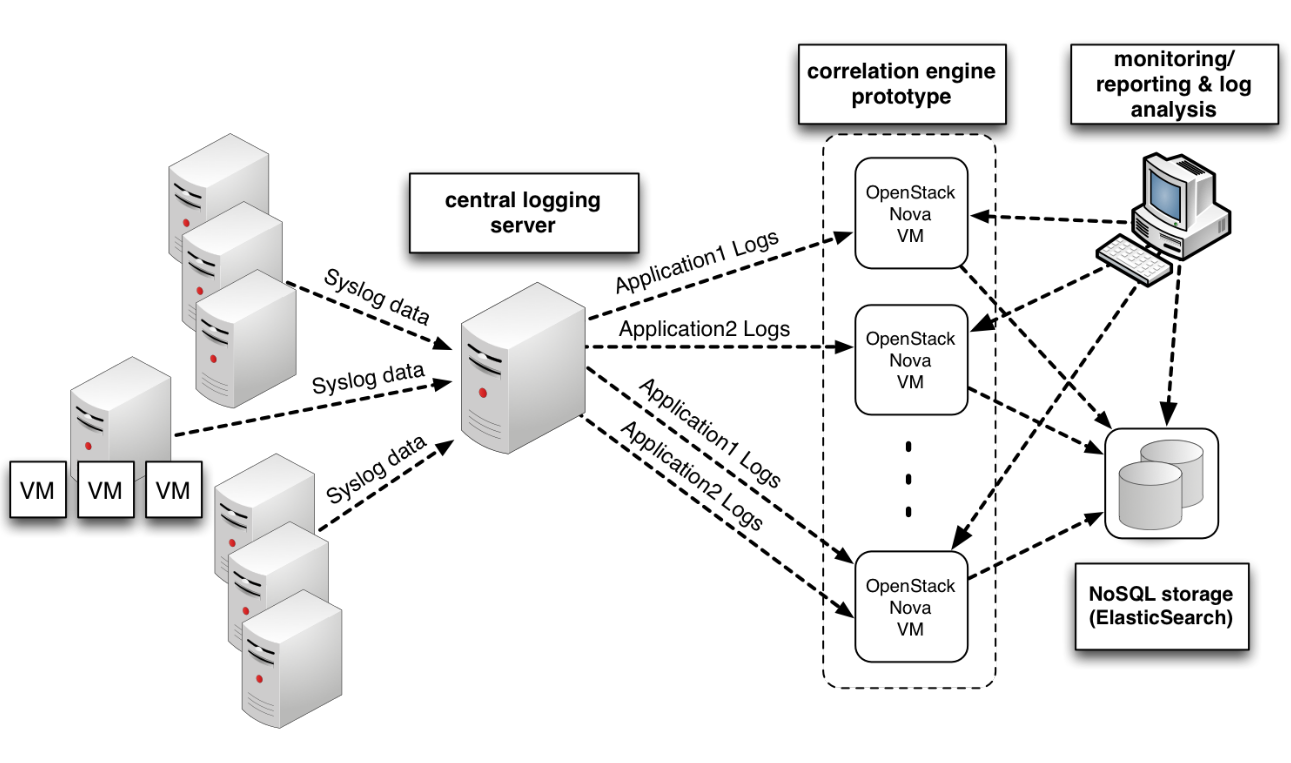
\includegraphics[scale=0.25]{img/schema_correlat-00.png}
\vspace{0.5cm}

\footnoterule
\footnotesize{
    Quelle:
    D.Frisch ,C. Pape, S. Reissmann, and S. Rieger “Correlation and
    Consolidation of Distributed Logging Data in Enterprise Clouds” In International
    Journal on Advances in Internet Technology, vol 7 , 2013, pp. 39–51.}

\end{frame}
%%%%%%%%%%%%%%%%%%%%%%%%%%%%%%%%%%%%%%%%%%%%%
\begin{frame}
\frametitle{Prototyp JCorrelat}
\framesubtitle{Schema}


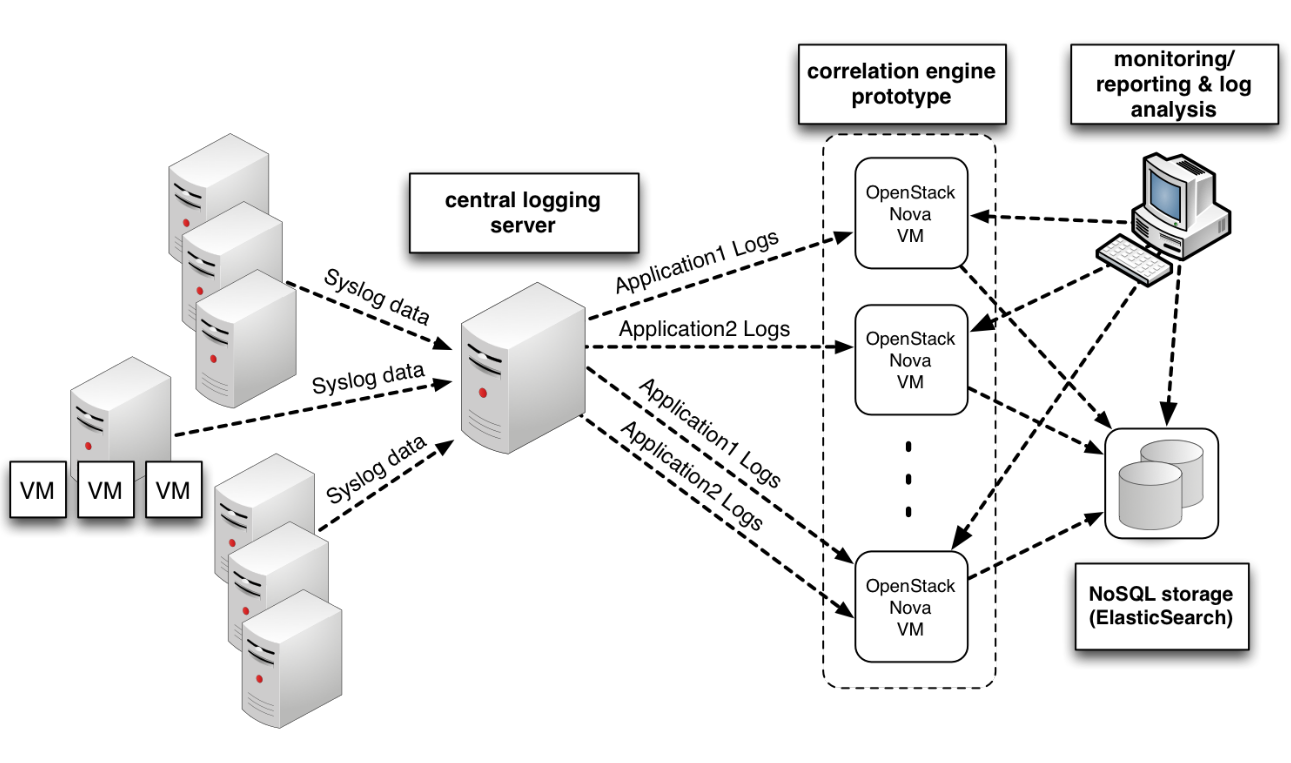
\includegraphics[scale=0.25]{img/schema_correlat-00.png}
\vspace{0.5cm}

\footnoterule
\footnotesize{
    Quelle:
    D.Frisch ,C. Pape, S. Reissmann, and S. Rieger “Correlation and
    Consolidation of Distributed Logging Data in Enterprise Clouds” In International
    Journal on Advances in Internet Technology, vol 7 , 2013, pp. 39–51.}

\end{frame}

\begin{frame}
\frametitle{Syslog}
\framesubtitle{Aufbau RFC 3164}
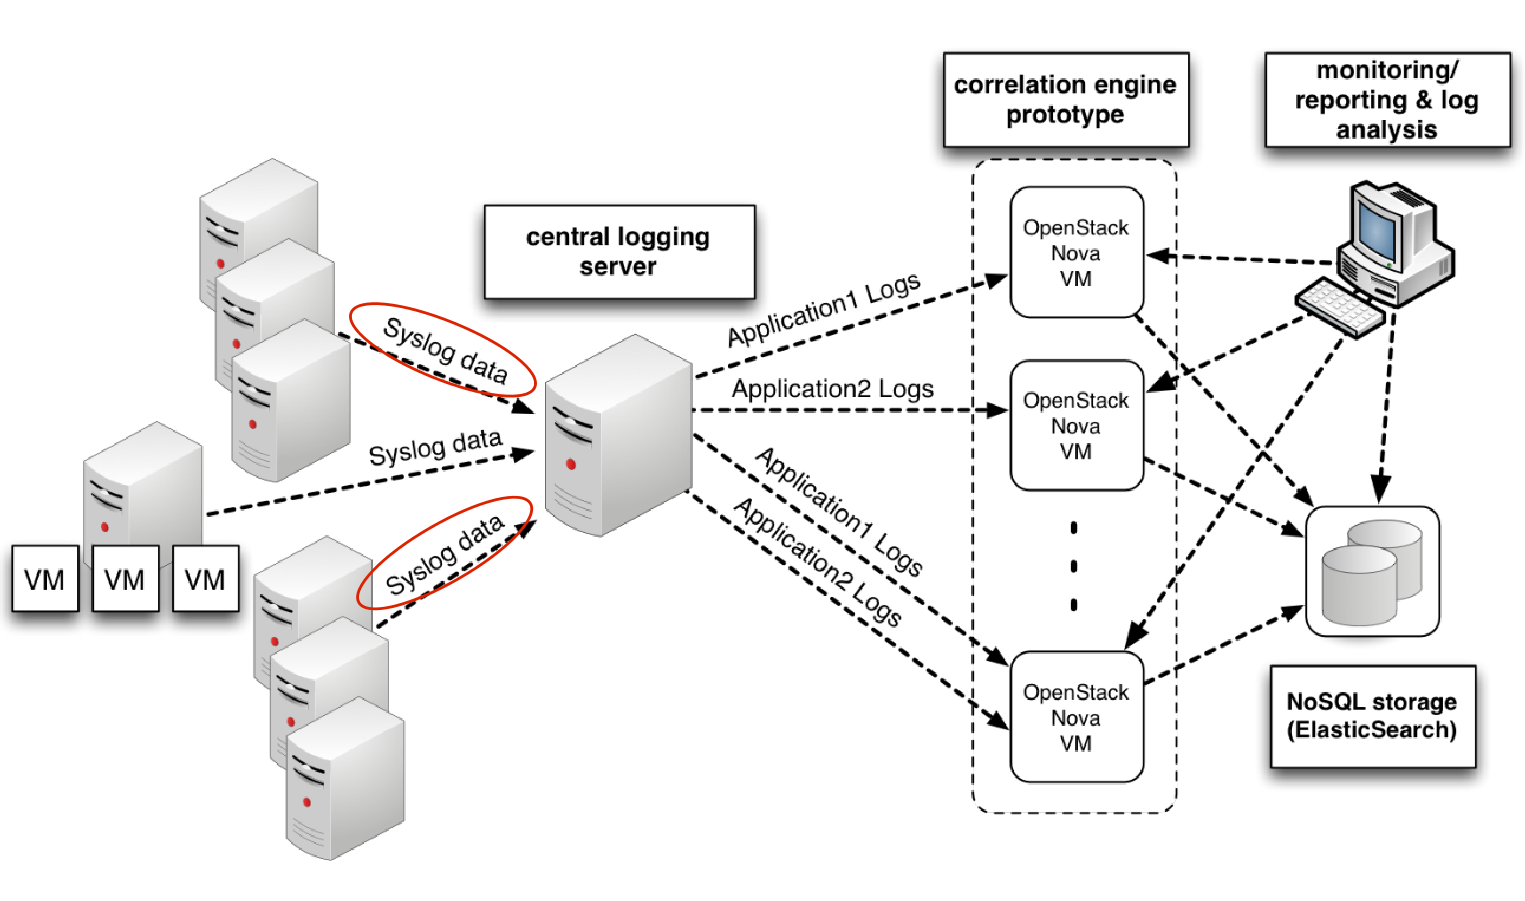
\includegraphics[scale=0.25]{img/schema-correlat-01.png}
\end{frame}


\begin{frame}[fragile]
\frametitle{Syslog}
\framesubtitle{Aufbau RFC 3164}

\begin{center}
\begin{tabular}{|l|c|c|}
  
    \hline 
    \zfA \textbf{Feld}&  \textbf{Inhalt}&
    \textbf{Beispiel}\\ 
    \hline
    \hline
    \zfB\multicolumn{3}{|l|}{PRI}\\
    \hline 
    \zfC facility & $int \in {0..23}$  & <\textbf{3}4> \\ 
    \hline 
    \zfC severity & $ int \in {0..7}$  &<3\textbf{4}>\\ 
    \hline
    \zfB \multicolumn{3}{|l|}{HEADER}\\
    \hline
    \zfC timestamp &mm dd hh:mm:ss  &\verb|Oct 11 22:14:15|\\ 
    \hline 
    \zfC hostname & string  &\verb|mymachine|\\ 
    \hline 
    \zfB \multicolumn{3}{|l|}{MSG}\\     
    \hline
    \zfC tag &string  &\verb|su:|\\
    \hline
    \zfC content &string&\verb|'su root' failed ...| \\
    \hline
\end{tabular} 
\end{center}

\vspace{0.5cm}
\small{
\begin{verbatim}
<34>Oct 11 22:14:15 mymachine su: 'su root' failed for lonvick
on /dev/pts/8
\end{verbatim}}

\end{frame}
\begin{frame}[fragile]
\frametitle{Syslog + strukturierte Daten}
\framesubtitle{Aufbau RFC 5425}

\centering{ \texttt{RFC5425} Implementiert durch \texttt{syslog-ng} und \texttt{rsyslog}}

\begin{center}
    \begin{tabular}{|l|c|c|}
        
        \hline 
        \zfA \textbf{Feld}&  \textbf{Inhalt}& \textbf{Beispiel}\\ 
        \hline
        \hline
        \zfB \multicolumn{3}{|l|}{HEADER}\\
        \zfC facility & $int \in {0..23}$  & <\textbf{16}5> \\ 
        \hline 
        \zfC severity & $ int \in {0..7}$  &<16\textbf{5}>\\ 
        \hline
        \zfD timestamp & \texttt{RFC3339}  &\verb|2003-10-11T22:14:15.003Z|\\ 
        \hline 
        \zfC hostname & string  &\verb|mymachine.example.com|\\ 
        \hline 
        \zfB \multicolumn{3}{|l|}{MSG}\\     
        \hline
        \zfC tag &string  &\verb|su:|\\
        \hline
        \zfC content &string&\verb|'su root' failed ...| \\
        \hline
    \end{tabular} 
\end{center}

\small{
\begin{verbatim}
<165> 2003-10-11T22:14:15.003Z mymachine.example.com
evntslog - ID47 [exampleSDID@32473 iut="3" eventSource=
"Application" eventID="1011"] BOMAn application
event log entry...
\end{verbatim}}

\end{frame}

%%%%%%%%%%%%%%%%%%%%%%%%%%%%%%%%%%%%%%%%%%%%%%%%%%%%%%%%%%%%%%%%%%%%%%%
%%%%%%%%%%%%%%%%%%%%%%%%%%%%%%%%%%%%%%%%%%%%%%%%%%%%%%%%%%%%%%%%%%%%%%%
\section{DEMO}
%%%%%%%%%%%%%%%%%%%%%%%%%%%%%%%%%%%%%%%%%%%%%%%%%%%%%%%%%%%%%%%%%%%%%%%
%%%%%%%%%%%%%%%%%%%%%%%%%%%%%%%%%%%%%%%%%%%%%%%%%%%%%%%%%%%%%%%%%%%%%%%
\frame{\tableofcontents[currentsection]}

%%%%%%%%%%%%%%%%%%%%%%%%%%%%%%%%%%%%%%%%%%%%%%%%%%%%%%%%%%%%%%%%%%%%%%%
\subsection{(Icinga2: aktives Monitoring)}
%%%%%%%%%%%%%%%%%%%%%%%%%%%%%%%%%%%%%%%%%%%%%%%%%%%%%%%%%%%%%%%%%%%%%%%
\begin{frame}
\frametitle{There Is No Largest Prime Number}

\end{frame}


%%%%%%%%%%%%%%%%%%%%%%%%%%%%%%%%%%%%%%%%%%%%%%%%%%%%%%%%%%%%%%%%%%%%%%%
\subsection{ELK-Stack: passives Monitoring}
%%%%%%%%%%%%%%%%%%%%%%%%%%%%%%%%%%%%%%%%%%%%%%%%%%%%%%%%%%%%%%%%%%%%%%%
\begin{frame}
\frametitle{There Is No Largest Prime Number}

\end{frame}

\end{document}

